\section{Notation and setting}\label{sec:background}
In this section, we present the relevant technical notation for the minimum violation synthesis problem in the UAM setting. 

%
\newcommand{\OperatorSpace}[5]{
				%\draw[rounded corners = 15pt,dashed] (#1-#4,#2-#5) rectangle (#1+#4,#2+#5);
		\fill[fill=green,opacity=0.2] (#1,#2) circle (#3);
		\draw[draw = black,dashed](#1,#2) circle (#3);
		%\node at (#1,#2-#5+0.5) {$\mathcal{T}_{#6}$};
	}
\tikzset{cross/.style={cross out, draw=black, minimum size=2*(#1-\pgflinewidth), inner sep=0pt, outer sep=0pt},
	%default radius will be 1pt. 
	cross/.default={4pt}}
	
\begin{figure}[h!]
	\centering
		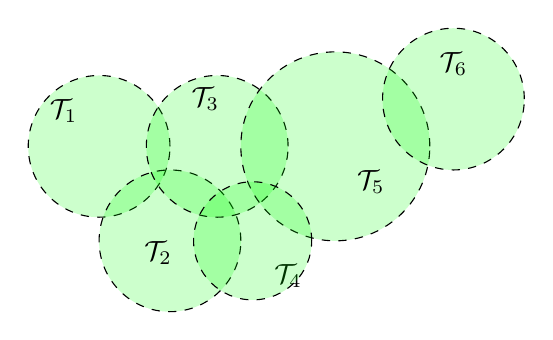
\begin{tikzpicture}[scale=0.3]
			\OperatorSpace{0}{0}{3}{5}{5}
			%\node at (-4.25,4.25){$S_1$};
			\node at (-1.5,1.5){$\mathcal{T}_1$};
			\OperatorSpace{3}{-4}{3}{5}{5}
			%\node at (-1.25,-8.25){$S_2$};
			\node at (2.5,-4.5){$\mathcal{T}_2$};
			%\node[red] at (2.5,3) (H13) {$H_{13}$};
			%\draw [->,red,line width = 0.75mm] (H13) -- (2.5,1.25);
			\OperatorSpace{5}{0}{3}{5}{6}
			%\node at (5-4.25,5.5){$S_3$};
			\node at (5-0.5,2){$\mathcal{T}_3$};
			%\node[red] at (6.5,3.5) (H35) {$H_{35}$};
			%\draw [->,red,line width = 0.75mm] (H35) -- (6.75,0.65);
			\OperatorSpace{10}{0}{4}{6}{7}
			
			\node at (8.5-0.5,-5.5){$\mathcal{T}_4$};
% 			\node[red] at (6.5,3.5) (H35) {$H_{35}$};
			%\draw [->,red,line width = 0.75mm] (H35) -- (6.75,0.65);
			\OperatorSpace{6.5}{-4}{2.5}{0}{0}
			
			%\node at (10+5.25,-6.5){$S_5$};
			\node at (10+1.5,-1.5){$\mathcal{T}_5$};
			\OperatorSpace{15}{2}{3}{5}{5}
			%\node at (15-4.25,5+3.25){$S_6$};
			\node at (15,3.5){$\mathcal{T}_6$};
			%\node[red] at (11,4.5) (H56) {$H_{56}$};
			%\draw [->,red,line width = 0.75mm] (H56) -- (12.5,2.75);

			
		\end{tikzpicture}
%		\setlength{\belowcaptionskip}{-2pt}
        \caption{Example UAM operating environment. Green circles correspond to the regions of vertihub controllers.}
	        \label{fig:RegionsOutline}
    \end{figure}

\subsection{Requests}
We define a request as a tuple $ O = \left(r,T,c \right)$ where
\begin{itemize}
    \item $r \in \mathcal{R}$ is the request class from a predefined set of classes $
    \mathcal{R}$. Request classes include \emph{landing at a particular vertiport in the region}, \emph{pass-through region}, \emph{take-off from vertiport in the region}. Depending on the nature of the problem, $\mathcal{R}$ can be defined to capture all types of desired outcomes for vehicles.   
    \item $T \in \mathbb{N}$ is the amount of time left before the request \emph{must} be granted. $t$ can function as an analogue for fuel reserves as vehicles requesting to land cannot hover indefinitely. 
    \item $c \in C$ is the class of UAM vehicle from a predefined set of vehicles $C$.  
\end{itemize}
At any given timestep $t$ the vertihub is managing requests from multiple vehicles.  We define the initial set of requests as the \emph{request allocation} and denote it as $\mathcal{O}^{\text{init}}$. We model the \emph{vertihub controller} that is responsible for managing these requests as a 
\emph{labeled weighted finite transition system}. 
\begin{eg}
Tower $\mathcal{T}_1$ is given a set of $N$ requests to handle $\mathcal{O}^{\text{init}} = \{O^{\mathcal{T}_1}_1 \dots O^{\mathcal{T}_1}_N \}$. For example, $O^{\mathcal{T}_1}_1 = \left(port\, A, 5, passenger \right)$ corresponds to a request by a \emph{passenger vehicle} trying to land at port A in \emph{at most} 5 time steps. 
\end{eg}




\subsection{Transition system model for vertihub controller}
Recall that in the previous section, I defined the vertihub and vertiport controller models as \emph{reactive systems}. However, in the case of minimum-violation planning, we focus purely on correctness with respect to finite-time linear temporal logic specifications. As such, the current methodology cannot yet handle the full expressiveness of the reactive system definition. For the purposes of the minimum-violation planning approach we henceforth model a vertihub controller is modeled as a tuple referred to as a labeled weighted finite transition system $\mathcal{T}_i = \left(S_i, s_{\text{init}_i},\Delta_i, \text{AP}_i,L_i \right)$ where

\begin{itemize}
    \item $S_i$ is a finite state space.  It is the set of all currently unapproved requests. Formally, if there are currently $m$ unapproved requests, we write $S_i = \{O_{i,1} \dots O_{i,m}\}$. We note that the state space can also include additional features of interest such as number of vehicles in the airspace, their landing/take-off statuses, and others. However, for notational simplicity we do not include these in the definition presented in this dissertation. In practice, these features, alongside the relevant modifications to the transition function, are straightforward to include. 
    \item $s_{\text{init}_i} \in S_i$ is the initial set of requests $\mathcal{O}^{\text{init}}_i$.
    \item $\Delta_i \subseteq S_i \times S_i$ is the deterministic transition function that governs how requests evolve. We have $\left(S^t_i,S^{t+1}_i \right) \in \Delta_i$ if:

    \begin{itemize}
        \item all \emph{approved} requests at timestep $t$, denoted $\mathcal O_{i,a}^t \subseteq S^t_i$,  are not present in $S^{t+1}_i$, i.e., if $O_{i,j} \in  \mathcal O_{i,a}^t$ then $O_{i,j} \notin S^{t+1}_i$, and
        \item all \emph{unapproved} requests at timestep $t$, denoted $S^{t}_i \setminus \mathcal O_{i,a}^t$, have their time remaining decremented, i.e., for all $O_{i,j} = (r,T,c)$ and $O_{i,j} \in S^{t}_i \setminus \mathcal{O}_{i,a}^t$, we will have $O_{i,j} \in S^{t+1}_i$ and $O_{i,j} = (r,\max(T-1,0),c)$. Informally, if request is not approved $\Delta_i$ decrements the remaining timer on the request by 1. 
    \end{itemize}
    \item $\text{AP}$ is a set of atomic propositions.
    \item  $L:S\rightarrow 2^{\text{AP}}$ is the labeling function.
\end{itemize}

Note that this is a much less general model than the reactive system approach. Handling the full expressiveness of reactive systems is a subject of future work in minimum-violation planning. 

At every timestep, the decision problem for the controller is to choose a set $O_{i,a}^t \subseteq S^{t}_i$ of requests to approve. The controller will also have the option to reroute the request to neighboring controllers

\begin{eg}
Consider vertihub controller $\mathcal{T}_1$ with two pending requests $O^{\mathcal{T}_1}_1 = \left(port\, A, 5, passenger \right)$ and $O^{\mathcal{T}_1}_2= \left(port\, A, 3, passenger \right)$. In this case, at time step $t$ we have $S_1^t = \{O_{1,1},O_{1,2}\}$ where $O_{1,1} = O^{\mathcal{T}_1}_1$ and $O_{1,2} = O^{\mathcal{T}_1}_2$. Let us assume at time step $t$ that the controller approves request $O_{1,2}$. We denote this as $\mathcal{O}^{t}_{1,a} = \{O_{1,2} \}$ and we will have $S^{t+1}_1 = \{O_{1,2}\}$ where $ O_{1,1} = \left(port\, A, 4, passenger \right)$. 
\end{eg}


A finite trace of $\mathcal{T}_i$ is a finite sequence of states $\tau_i = s_{i,0} s_{i,1} \ldots s_{i,n}$ such that
$s_{i,0} = s_{\textit{init}_i}$ and $(s_{i,j}, s_{i,j+1}) \in \Delta_i$, for all $j \in \mathbb{N}_{\leq n-1}$.
A finite trace $\tau = s_0 s_1 \ldots s_n$ produces a finite word $w(\tau) = L(s_0) L(s_1) \ldots L(s_n)$. For any $s \in S$, we let $\text{Traces}(\mathcal{T}, s)$ represents the set of all finite traces of $\mathcal{T}$ that ends with $s$.

The aim of the transition system $\mathcal{T}_i$ is to reach a \emph{goal state} denoted $s_{\text{final}} \in S_i$. Since the hub controller needs to eventually grant all requests, $s_{\text{final}}$ corresponds to the state with no more pending requests. Formally, we have $s_{\text{final}} = \emptyset$.  

The goal of this approach is to synthesize a trace for each vertihub such that requests are accepted in a manner that satisfies all regulations. However, if this is not possible, it must approve requests in a way that minimally violates regulations. we employ linear temporal logic due to its ability to formally express a wide array or requirements. Specifically, we employ finite linear temporal logic (FLTL) to precisely describe the safety-oriented regulations. Note this FLTL has been used in the context of autonomous driving to formally represent road safety laws for planning~\cite{Tumova:2013:ACC,Tumova:2013:LCS}. 

\subsection{Finite linear temporal logic}
An FLTL formula is built up from the same logical notation as the LTL formulas defined earlier. The main point of contrast is that an FLTL formula $\psi$ over a set $\text{AP}$ of atomic propositions is interpreted over a finite word
$w = l_0 l_1 \ldots l_n \in (2^{\text{AP}})^{n+1}$,
and we write $w \models \psi$ if $w$ satisfies $\psi$.
In particular, consider $p \in \text{AP}$. Then,
$w \models p$ if and only if $p \in l_0$. Also,
$w \models \square p$
if and only if $p \in l_i$ for all $i \in \{0, \ldots, n\}$. Please refer to~\cite{gunter2002temporal} for full FLTL semantics. 

\begin{eg}
 14 CFR \S 107.49 (d) requires the vehicle to have enough power for its operations and hence, a vertihub cannot force a vehicle to loiter for too long. We can capture this as a specification $\psi = \square \{\lnot fuel\_too\_low_i\} $ where $fuel\_too\_low_i$ is an atomic proposition that is true when request $O_i = (r,T,c)$ has $T = 0$.
\end{eg}



A \emph{non-deterministic finite automaton} (NFA) is a  tuple $\mathcal A = (Q,q_{\text{init}},\Sigma,\delta,F)$ where $Q$ is a finite set of states; $q_{\text{init}} \in Q$ is the initial state; $\Sigma$ is the input alphabet; $\delta \subseteq Q \times \Sigma \times Q$ is a non-deterministic transition relation; and $F \subseteq Q$ is the set of accepting states. 

Given an input word $w = w(1),\dots,w(n)$, a \emph{run} of $\mathcal A$ is a sequence $\rho = q_0q_1,\dots,q_n$, such that $q_0 = q_{\text{init}}$, and $q_{i-1},w(i),q_i \in \delta$ for all $1 \leq i \leq n$. We say a run is \emph{accepting} if $q_n \in F$. It can be shown that for any given FLTL formula $\varphi$ over $\text{AP}$, there exists an NFA $\mathcal{A}$ with alphabet $\Sigma = 2^{\text{AP}}$ that accepts all and only words over $\text{AP}$ that satisfy $\varphi$. Automatic translation of FLTL to NFA is proposed in \cite{}.

A \emph{weighted non-deterministic finite automaton} is a tuple $\mathcal A = (Q,q_{\text{init}},\Sigma,\delta,F,W)$ where $Q$, $q_{\text{init}}$, $\Sigma$, $\delta$ and $F$ are defined as those in the NFA and $W : \delta \rightarrow \mathbb{N}^k$, where $k \in \mathbb{N}$ is a weight function.  

Consider now a run $\rho$ in automaton $\mathcal A$ over a word $w \in \Sigma^{n}$. Let $\left(c_{i,1},c_{i,2},\dots,c_{i,k}\right) = W(q_{i},w(i),q_{i+1})$ denote the weight of the transition $\delta(q_{i},w(i),q_{i+1})$ for all $i = 1,\dots,n$. The weight of the full run $\rho$ is the component-wise sum of the weights of each transition on the run. Formally, $W(\rho) = \left(C_1,\dots,C_k \right)$, where $C_i = \sum_{j=0}^n c_{i,j}$.




\subsection{Prioritized safety specification}
A \emph{prioritized safety specification} is a tuple
$\mathcal{P} = (\text{AP}, \Omega, \Psi, \varpi)$ where
$\text{AP}$ is a set of atomic propositions,
$\Omega$ is a set of FLTL formulas over $\text{AP}$,
$\Psi = (\Psi_1, \Psi_2, \ldots, \Psi_N)$,
$\Psi_i \subseteq \Omega$
for all $i \in \{1, \ldots, N\}$,
and
$\varpi : \Omega \to \mathbb{N}$
is the priority function that assigns the weight to each
$\psi \in \Omega$.

\begin{eg}\label{ex:prioritized safety}
 A potential prioritized safety specification $\Psi = \{\Psi_1,\Psi_2\}$ for a vertihub to satisfy is $\Psi_1 = \{\psi_{1,1}\}, \Psi_2 = \{\psi_{2,1}, \psi_{2,2}, \psi_{2,3}\}$ where %\textbf{\textcolor{blue}{Write FLTL specs for these}}
\begin{itemize}
    \item $\psi_{1,1}$ = Never allow the timer on a request to expire. 
    \item  $\psi_{2,1}$ = Do not land vehicles past a vertiport's capacity.
    \item  $\psi_{2,2}$ = Do not allow more than $M$ vehicles in the vertihub's airspace at a time.
    \item  $\psi_{2,3}$ = Do not land a vehicle at a vertiport it did not request.
\end{itemize}
\end{eg} 

Note that the requirements at level i are strictly more important than those at level i+1, i.e., the system first attempts to minimize the amount of violation of level-1 requirements. Then among all the policies that minimize the violation of level-1 requirements, it attempts to minimize the amount of violation of level-2 requirements, and so on. In Example~\ref{ex:prioritized safety}, the first specification is the highest priority and the remaining specifications are all of equal priority. We use this example in the case study detailed in the Experimental Results section.

\subsection{Lack of safety}
Consider an FLTL formula $\psi$ over $\text{AP}$ and a finite word $w = l_0 l_1 \ldots l_n \in (2^{\text{AP}})^{n+1}$.
The \emph{lack of safety} of $w$ with respect to $\psi$ is defined as
\begin{equation}
        \lambda(w, \psi) = \min_{I \subseteq \mathbb{N}_{\leq n} |
        \mathsf{vanish}(w, I) \models \psi}
        |I|,
\end{equation}
where for any given finite sequence $w = l_0 l_1 \ldots l_n$
and a set $I \subseteq \mathbb{N}$,
$\mathsf{vanish}(w, I)$ is defined as a subsequence of $w$ obtained by
removing all $l_i$, $i \in I$.

Let $\mathcal{P} = (\text{AP}, \Omega, \Psi, \varpi)$ be a prioritized safety specification where $\Psi = (\Psi_1, \Psi_2,$ $\ldots, \Psi_N)$.
We define the \emph{lack of safety} of $w$ with respect to $\mathcal{P}$ as
\begin{equation}
        \lambda(w, \mathcal{P}) = (\lambda(w, \Psi_1), \ldots, \lambda(w, \Psi_N))
        \in \mathbb{N}^{N},
\end{equation}
where for each $i \in \{1, \ldots, N\}$,
\begin{equation}
        \lambda(w, \Psi_i) =
        \sum_{\psi \in \Psi_i} \varpi(\psi) \lambda(w, \psi).
\end{equation}

Note that there are two mechanisms to address the unequal importance of safety specifications. Namely, the prioritization of specifications by $\Psi$ and the weighting function $\varpi(\psi)$.  The weights $\varpi$ indicates the importance among different requirements within the same level.

The lack of safety of a trace $\tau$ of a finite transition system with respect to $\mathcal{P}$
is defined based on its produced word, i.e., $\lambda(\tau, \mathcal{P}) = \lambda(w(\tau), \mathcal{P})$.
The standard lexicographical order is used to compare the lack of safety between different traces.

\paragraph{Remark}
There are two mechanisms to specify the unequal importance of different specifications, the hierarchy $(\Psi_1, \Psi_2, \ldots, \Psi_N)$ and the weights captured by $\varpi$.
As the standard lexicographical order is used to compare the lack of safety between different traces, the algorithm first minimizes the lack of safety with respect to the specifications in $\Psi_1$.
Then, among all the traces that minimizes the lack of safety with respect to $\Psi_1$, it minimizes the lack of safety with respect to the specifications in $\Psi_2$, and so on.
The weights $\varpi$ only matter for the specifications within the same level of hierarchy.